% Here comes the helicene paper
\label{section:helicene}
\section{Abstract}

We propose the novel synthetized 7,8-dicyano-5,6,9,10-dibenzo-[5]Helicene (dcdb-[5]H) as model compound to investigate intermolecular interactions present for chiral, dipolar species. The adsorption on different metal surface terminations (Ag(111)/Ag(100)) shows the importance of the cyano group. It determines the orientation of dcdb-[5]H strands along the substrate's high symmetry directions and dominates the intermolecular coupling of constructive enantiomers resulting in parallel dipole orientation. While on metal substrates strands are paired depending on the surface termination, broad islands are achieved by introducing a monolayer of \textit{h}-BN grown on Cu(111) maintaining strands as building blocks but lifting their substrate interactions. On this geometrically flat surface, molecular orbital energies align to the modulated surface potential arising from the superstructure present in this lattice mismatched system. Here interactions between molecular and STM-tip dipole are observed.

\section{Introduction}

To gain insight in intermolecular interactions present on a sub-molecular level, model systems used are often reduced to two dimensions. This can be achieved by adsorption on a surface under UHV conditions that guarantee a clean chemical environment. vdW interactions can be investigated with high precision for molecules that consist of simple hydrocarbon species to help analyze larger, more complicated systems. 
While homogenously charged species govern their assembly by vdW interactions and avoidance of steric hinderance (pauli repulsion), polar molecules exhibit additional dipole interactions. The importance of these is evidenced for fluorenone derivatives \cite{Cui_Self-assembly_2015, Xu_Dipole-controlled_2013, Xu_Two-dimensional_2012}, hydroxyanthraquinone\cite{Hu_Structural_2016}, octanoic acid \cite{Hu_Effects_2017} and thiopene derivatives \cite{Heller_Self-assemlby_2012} on HOPG surfaces where the combined interplay between extended alkyl chains and dipole moment forms columns and two-dimensional packings. Repulsive and attractive forces determine the assembly of anthracenes with ether side chains and cause a patterned monolayer to form\cite{Wei_Dipolar-control_2006}.  Depending on the substrate, dipole moments have shown the ability to overcome electrostatic interaction energies to form gratings and 2D islands.\cite{Kunkel_Self-assembly_2015}

Progress in coordination chemistry led to a variety of processes to heavily modify molecules or to completely design them on the drafting table by the needs of the task. It was shown that supramolecular structures of Hexa-peri-hexabenzocoronene with CN and NO2 groups form hexagonal assemblies while functionalization with CF3 groups opens a porous honeycomb structure under the influence of the larger dipole moment.\cite{Mu_Effect_2011}

Since the mid 50’s of the last century helicenes faced increasing interest in their chiral and optical properties.\cite{Newman_synthesis_1956, Rau_Exciplex_1992, Donckt_Flourescence_1968} Helicenes consist of ortho-condensed, six membered carbon rings annulated at position 1 \& 2 to form circular structures. Due to overcrowding in their center spirals are formed. Depending on the turn direction two enantiomers can be distinguished denoted as “R” [lat.: rectus, right] and “S” [lat.: sinister, left], often noted as P(lus) and M(inus). Like left and right turning screws, these are related to each other like mirror images that cannot be superimposed by rotation or translation. The lack of a rotary reflection axis is what makes these molecules chiral, an interesting geometric property present in many biological entities like sugars and proteins determining their biological function. 

Because in simple helicenes carbon atoms are passivated with hydrogen, stereo selective molecular recognition mediated by van der Waals (vdW) forces plays an important role for 2D conglomerate crystallization.\cite{Treier_aromatic_2008} (S)-proline, an amino acid, shows extended 2D island growth of enantiopure molecules, consisting of hydrogen bonded chains on a Cu(110) surface.\cite{Forster_Probing_2009} On the same surface the self-assembly of adenine is guided by hydrogen bonds to form linear and ladder like chains\cite{Cheng_Role_2016} and meta-aminobenzoate molecules assemble through hydrogen bonds between amino groups and carboxylate groups.\cite{Rabot_Self-assembly_2009}

The subtle interplay of hydrogen bonds, vdW- and dipole interactions can be accessed by designed chemical substituents that steer molecular assembly and function via their type, number and position in the molecule. Dibenzo-5[H] was used as model system to understand diastereomeric interactions in 2D crystals formed on an Au(111) surface where molecules deposited at room temperature (RT) form heterochiral 2D conglomerates.\cite{Seibel_Chiral_2013} (Molecular motion is frozen below 50K where only homochiral molecular domains are observed.) Enantiopure 6,13-dicyano[7]H was used to study chiral recognition and chirality transfer on Cu(111)\cite{Shchyrba_Chirality_2013, Stoehr_Self-assembly_2011}, where the presence of the polar cyano group guides chain formation oriented 30° off the Cu(111) high-symmetry directions at lower coverages and forms 2D agglomerates at higher coverage. While close packing on single-crystal surfaces is always a combination of intermolecular forces and occupation of the favored ad-sites at saturation coverage, molecules may behave different when adsorbed on different surfaces. The interplay of surface and helicenes’ molecular structure is important for stereochemical recognition\cite{Ernst_Stereochemical_2016} and already investigated on (111) surfaces of silver and gold\cite{Seibel_Two-dimensional_2014} and Ag(100)\cite{Seibel_Homochiral_2015}. To understand enantiomorphism in 2D molecular crystals heptahelicene ([7]H) is used.\cite{Parschau_coverage_2008, Fasel_Amplification_2006} On Cu(100) 2D conglomerate crystallization leads to homochiral domains\cite{Seibel_conglomerate_2014} while racemic crystals\cite{Fasel_Amplification_2006} and separated homochiral domains\cite{Ernst_two-dimensional_2001} are reported on Cu(111) where substantial vdW repulsion was presumed. For enantiopure [7]H a transfer of molecular chirality into a long-range chirality of the assembled molecular assembly is observed on Cu(111)\cite{Fasel_Chirality_2003} and second layer adsorption leads to quasi-epitaxial growth with chirality transfer occurring in 3D.\cite{Parschau_Chirality_2010}

Not only acts the metal surface as a guide for 2D molecular motion, it is also an almost infinite charge supply/drain. With neglect able DOS close to the fermi energy, a single layer of hexagonal boron nitride (\textit{h}-BN) acts as isolating spacer layer and reduces the influence of the substrate on the molecular assembly and frontier orbitals.\cite{urgel_controlling_2015, Sushobhan_Control_2014, Schulz_Templated_2013} With a lattice mismatch of (2\%)\cite{joshi_boron_2012, preobrajenski_monolayer_2005} the geometrically flat\cite{schwarz_corrugation_2017} \textit{h}-BN adlayer forms a electronically corrugated superstructure (moir\'e) on Cu(111).\cite{joshi_boron_2012} Here the surface potential is nano-patterned\cite{joshi_boron_2012}, following the substrate’s hexagonal symmetry, with the period determined by the angle between \textit{h}-BN and Cu(111)\cite{hermann_periodic_2012}. The surface potential influences the energy of highest occupied (HOMO) and lowest unoccupied (LUMO) molecular orbital with respect to the vacuum level.\cite{Sushobhan_Control_2014, Fernandez_Spectroscopy_2008} STM is a versatile tool to investigate those systems since it detects geometric as well as electronic properties, and is even able to follow Ullmann coupling of bishelicenes on Cu(100)\cite{Waeckerlin_Surface-assisted_2016} on the surface. 

\paragraph{The molecule}

In this work we investigate sub-monolayer coverages of 7,8-dicyano-5,6,9,10-dibenzo-[5]Helicene (dcdb-[5]H). The benzol groups condensed at positions 5,6,9,10 to the five carbon rings of [5]H (db-[5]H) are used to achieve a more distinct footprint of the molecule. Two cyano groups added at the central carbon ring induce a permanent dipole moment of 6.3 D (\autoref{fig:hel-fig1}a,b) and complete the molecule we use here. It is adsorbed @ RT on 1. a thin, insulating hexagonal boron nitride monolayer grown on a copper single crystal (\textit{h}-BN/Cu(111)) as well as 2. different surface terminations of a metallic silver single crystal (Ag(111) \& Ag(100)). The preparations are investigated with scanning tunneling microscopy \& spectroscopy @ 5K (LT-STM/STS).

\begin{figure} \centering
	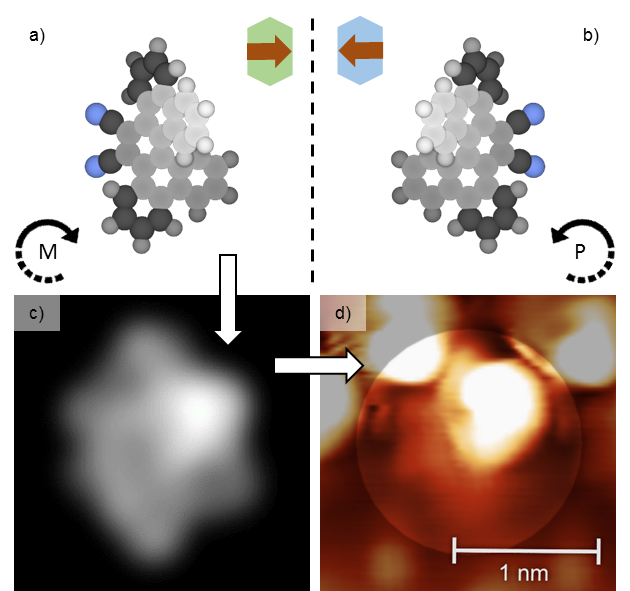
\includegraphics[width=0.7\textwidth]{./images/paper/helicene/fig1}
	\caption{Representations of dcdb[5]-H. Ortho-fused carbon rings build a helical structure which results in a chiral nature of this molecule. a, b) Ball models with indication of the chiral nature. The molecule either turns up clockwise (green hexagon, M) or counter clockwise (blue hexagon, P). A large dipole moment (orange arrow) is build up through the functionalization with two cyano groups at the central carbon ring. c) EHT simulated STM image of the M enantiomer. d) LT-STM image of an M enantiomer on Ag(111). All images show \SI{2}{\nano \meter} $\times$ \SI{2}{\nano \meter}, Image d is recorded at \SI{150}{\milli \volt}, \SI{0.09}{\nano \ampere}.}
	\label{fig:hel-fig1}
\end{figure}

The carbon backbone of dcdb-5[H] either turns up clockwise (denoted as ‘M’) or counter-clockwise (‘P’) and is therefore chiral as shown in \autoref{fig:hel-fig1}a,b. The color of the carbon atoms in the helicene backbone emphasizes their height and allows for easier recognition of the turn direction also indicated by the circular arrows. The hexagons (green in \autoref{fig:hel-fig1}1a for the M enantiomer and blue in \autoref{fig:hel-fig1}b for the P enantiomer) resemble the footprint of the molecule, while the direction of the dipole moment is indicated by an orange arrow within. To identify the adsorption geometry via LT-STM imaging, extended Hückel calculations are performed. A comparison between calculated (\autoref{fig:hel-fig1}c) and measured (\autoref{fig:hel-fig1}d) STM image of the M enantiomer shows that one benzol-group at the lower part of the helicene backbone  adsorbs flat on the Ag(111) surface while the opposing end of the helicene screw points away from the surface – a geometry reported for helicenes on other metal surfaces, too.\cite{Fasel_Orientation_2001} This distal part of the molecular helix is imaged as protrusion in STM and is the dominant distribution to the STM contrast in all images. The benzol groups are recognized as darker regions with uniform contrast to the sides while the cyano group contributes barely to most of the observed contrasts in STM. A match between calculated and measured STM image can only be obtained in the shown configuration (\autoref{fig:hel-fig1}a-c) allowing for assignment of chirality and azimuthal orientation on the surface.

\section{Results \& discussion}
\subsection{on Ag(111)}
\begin{figure} \centering
	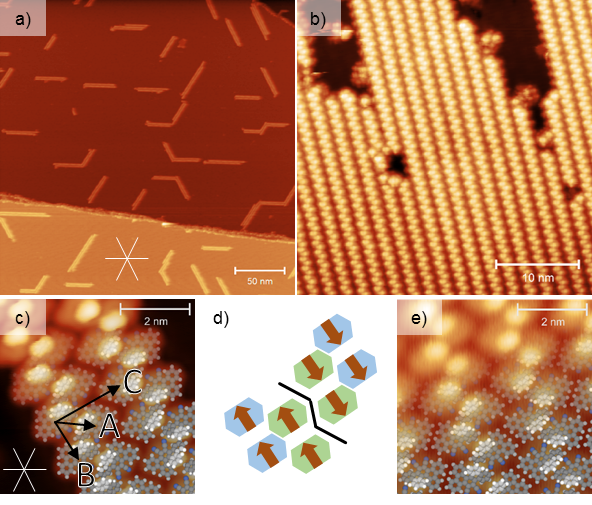
\includegraphics[width=0.7\textwidth]{./images/paper/helicene/fig2}
	\caption{Dcdb-[5]H on Ag(111) (a) and on \textit{h}-BN/Cu(111) (b). Detail images of a chain and parts of the extended island are shown in c) and e) respectively. Labelled arrows in c) indicate the direction in which center-center distances have been measured. A model representation of the binding motif is given in d). It shows a simplified representation of the models overlaid in c) and e). High symmetry directions for Ag(111) are depicted as white lines. The binding motif is the same in both cases though extended islands only form on \textit{h}-BN. Imaging parameters: 
		a) %295 nm x 295 nm, 655 mV, 0,02 nA,
		\SI{295}{\nano \meter} $\times$ \SI{295}{\nano \meter},
		\SI{655}{\milli \volt}, \SI{0.02}{\nano \ampere} 
		b) %35 nm x 35 nm, 2.37 V, 0.13 nA, 
		\SI{35}{\nano \meter} $\times$ \SI{35}{\nano \meter},
		\SI{2.37}{\volt}, \SI{0.13}{\nano \ampere}
		c) %5.5 nm x 5.5 nm, -500 mV, 0.1 nA, 
		\SI{5.5}{\nano \meter} $\times$ \SI{5.5}{\nano \meter},
		\SI{-500}{\milli \volt}, \SI{0.1}{\nano \ampere}
		e) %5.5 nm x 5.5 nm, 1 V, 0.07 nA.}
		\SI{5.5}{\nano \meter} $\times$ \SI{5.5}{\nano \meter},
		\SI{1}{\volt}, \SI{0.07}{\nano \ampere}
	}
	\label{fig:hel-fig2}
\end{figure}

To clarify the molecular interaction geometries within the assembly, dcdb-[5]H is adsorbed on Ag(111) (\autoref{fig:hel-fig2}a,c).  It assembles in 1D-chains oriented along the high symmetry directions of the three-fold symmetric substrate. A typical chain contains between \SIrange{30}{50}{}molecules (compare appendix \autoref{fig:hel-figS3}). Each chain is made up two single strands. The model representation (\autoref{fig:hel-fig2}d) partially shows two strands of a chain separated by a black line. A strand consists of molecules with alternating chirality but parallel aligned dipole moment. Two strands rotated by \SI{180}{\degree} with respect to each other form the chain shown in \autoref{fig:hel-fig2}c. The inter-molecular distance (center-center) of neighboring molecules with different chirality is $A_{Ag(111)}$ = \SI{0.81 \pm 0.06}{\nano \meter}, two molecules with the same chirality are separated by $B_{Ag(111)}$ = \SI{1.21 \pm 0.06}{\nano \meter}. Single strands are $C_{Ag(111)}$ = \SI{2.09 \pm 0.06}{\nano \meter} apart. The close arrangement of the molecules in a strand is possible because the cyano groups of the molecule have a lower height than the elevated carbon ring of its closest chiral counterpart. Although – if like here the geometry is projected orthographically onto the surface – the molecules seem to touch this is not the case. The same is true for two elevated carbon “tails”. Their elevation leads to carbon rings with a well-defined distance. Only the projection on the image plane makes them look closer than they are in real space. If a chain happens to have a kink both parts of the chain follow the high symmetry directions of Ag(111). The connection point of two chains is made such that frontier molecules of different chains connect with their cyano groups always pointing towards the helicene backbone of the connecting chain. Most chains terminate with the same length of their constituting strands pointing to a mechanism where the total dipole moment of the chains is minimized. The fact that chains on Ag(111) almost exclusively occur in pairs of strands (even number of molecules in chain width (\autoref{fig:hel-fig-S3})) underpins this assumption and leads to a minimum of total surface dipole. Molecules are stable upon annealing to \SI{100}{\celsius}. LT-STM images for an annealing sequence from \SIrange{100}{175}{\celsius} can be found in the appendix (\autoref{fig:hel-fig-S1}) depicting the gradual decrease in chain length and over all order. The longer the annealing time, the more pronounced this effect gets. When exceeding an annealing temperature of \SI{100}{\celsius} a surface assisted, temperature induced cyclodehydrogenation is observed (\autoref{fig:hel-fig-S2} in appendix) for a fraction of molecules that increases with temperature and time. Here the first and last ring of the helicene backbone fuse together, forming a flat molecule with no chiral properties. This new compound tends to form separate chains often attached to existing ones. 

\subsection{on \textit{h}-BN on Cu(111)}
To further investigate the intermolecular interactions dcdb-[5]H is adsorbed on \textit{h}-BN/Cu(111). Here extended islands (\autoref{fig:hel-fig2}b,e) are formed. The building block of this 2D assembly is the same as after adsorption an Ag(111) (i.e. strands) which can still be recognized at the edges of the assembly. Several strands form an island, where again every second strand is rotated by \SI{180}{\degree}. Different islands on the same \textit{h}-BN flake do not show a fixed orientation to the underlying substrate (not shown here). Distances are $A_{\textit{h}-BN}$ = \SI{0.77 \pm 0.06}{\nano \meter}, $B_{\textit{h}-BN}$ = \SI{1.20 \pm 0.06}{\nano \meter} and $C_{\textit{h}-BN}$ = \SI{2.05 \pm 0.06}{\nano \meter} - close to those on Ag(111). On \textit{h}-BN the molecules assemble the same way as on a metallic support. This suggests that the molecule-substrate interaction is weaker than the inter-molecular interaction including 1: hydrogen-bridge bonding of CN- groups towards the terminal H of the next molecule (along A \& B), 2: $\pi$-stacking of molecular orbitals of elevated carbon rings (along A), 3: vdW interactions of flat helicene parts (between chains, along C) and 4: dipole interaction along direction B (parallel within strands) \& C (antiparallel for neighboring strands).  Strict orientation of the molecular assembly along the crystal axis on metal supports indicate an interaction between the molecule (functional –CN group) and the substrate. This restriction is lifted when changing to the insulating \textit{h}-BN support leading to coincidentally oriented molecular islands.

\subsection{on Ag(100)}

\begin{figure} \centering
	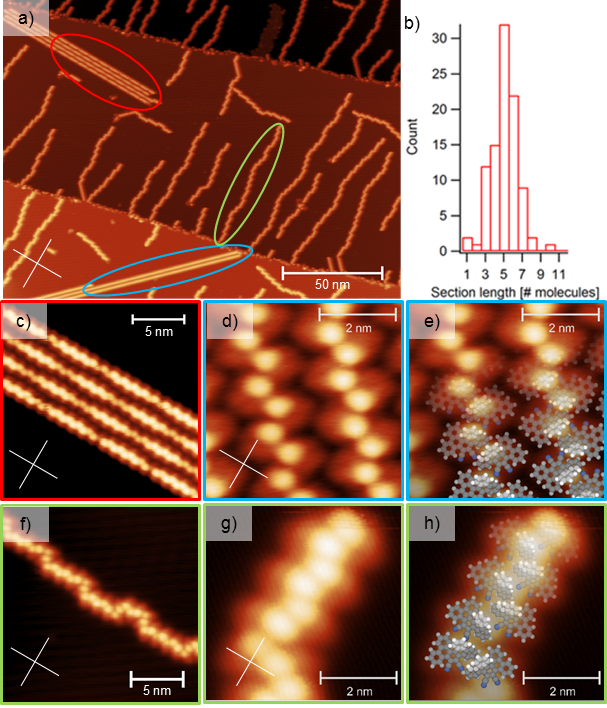
\includegraphics[width=0.7\textwidth]{./images/paper/helicene/fig3}
	\caption{Self-assembled structures upon RT adsorption on Ag(100). White lines show the high symmetry directions of the substrate. A statistical analysis of the section length of kinked strands is shown in b). Overview (f) and detail images (g, h) show the binding motif within kinked strands. Broad chains are observed less often. Those aligned along [0 1 1] \& [0 -1 1] (c) show periodic height modulation. Chains oriented along [0 0 1] \& [0 1 0] (d, e) do not show periodic height modulation. Imaging parameter: 
		a) %200 nm x 150 nm, 500 mV, 0.04 nA, 
		\SI{200}{\nano \meter} $\times$ \SI{150}{\nano \meter},
		\SI{500}{\milli \volt}, \SI{0.0}{\nano \ampere} 
		c) %18 nm x 18 nm, 450 mV, 0.2 nA, d,
		\SI{18}{\nano \meter} $\times$ \SI{18}{\nano \meter},
		\SI{450}{\milli \volt}, \SI{0.2}{\nano \ampere} 
		e) %5 nm x 5 nm, 31 mV, 0.5 nA,
		\SI{5}{\nano \meter} $\times$ \SI{5}{\nano \meter},
		\SI{31}{\milli \volt}, \SI{0.5}{\nano \ampere}  
		f) %18 nm x 18 nm, 272 mV, 0.06 nA,
		\SI{18}{\nano \meter} $\times$ \SI{18}{\nano \meter},
		\SI{272}{\milli \volt}, \SI{0.06}{\nano \ampere}  
		g,h) %5 nm x 5 nm, 325 mV, 0.1 nA
		\SI{5}{\nano \meter} $\times$ \SI{5}{\nano \meter},
		\SI{325}{\milli \volt}, \SI{0.1}{\nano \ampere} 
	}
	\label{fig:hel-fig3}
\end{figure}

We prepared dcdb-[5]H on Ag(100) to further investigate the influence of the substrate termination on the molecular self-assembly. Ag(100) has two different sets of symmetry directions in a square unit cell. Directions [0 1 1] \& [0 -1 1] point from one surface atom to its nearest neighbor (white lines in \autoref{fig:hel-fig3}). [0 0 1] \& [0 1 0] are rotated by \SI{45}{\degree} with respect to [0 1 1] \& [0 -1 1] and point from one surface atom to its second nearest neighbor. \autoref{fig:hel-fig3}a is an overview STM image showing different chain orientations (i-iii) where three of them are marked with colored ellipses. Enlarged views (c,d,f,g) and overlaid atomic models (e,h) are given with the corresponding color frame. Like on Ag(111) molecules assemble in chains oriented along the high symmetry directions. Type i) chains aligned along [0 1 1] \& [0 -1 1] (red) show modulation of their apparent height visible in STM (\autoref{fig:hel-fig3}c). The period of this modulation is \SI{6.03 \pm 0.11}{\nano \meter}. For these, differential conductance (dI/dV) maps are recorded at voltages ranging from \SIrange{0.3}{0,6}{\volt} (see appendix \autoref{fig:hel-fig-S5}) showing the lateral distribution of the corresponding molecular states. These show a similar period of \SI{6.1 \pm 0.3}{\nano \meter}. Both indicate a commensurate growth (every 12th dcdb-5[H] molecule occupying the same lattice site every 21st silver surface atom - corresponding to a period of \SI{6.048}{\nano \meter}. This is in line with the molecule-substrate interaction visible in the strict alignment of molecular and crystal axis. It is likely that the two -CN groups of the molecule determine the commensurate adsorption position and the registry to the substrates’ high symmetry directions. 

The reduced surface symmetry results in additional assemblies (ii-iii) not observed on Ag(111) or \textit{h}-BN/Cu(111). ii) Some chains are oriented along [0 0 1] \& [0 1 0] (blue ellipse in \autoref{fig:hel-fig3}d,e). The distances in this molecular assembly are $A^b_{Ag(100)}$ = \SI{0.67 \pm 0.06}{\nano \meter}, $B^b_{Ag(100)}$ = \SI{1.25 \pm 0.06}{\nano \meter} and $C^b_{Ag(100)}$ = \SI{2.10 \pm 0.06}{\nano \meter}. These do not show modulation in apparent height. iii) The majority of the chains is formed by a single strand, which is oriented along [0 1 1] \& [0 -1 1] and periodically kinked. The cyano group always points towards a rising step edge if connected to one. If a strand kinks to the left or right is defined relative to the direction of its dipole moment. The kinked nature results in 1: a connecting segment between two sections, 2: a turn direction for each kink and 3: a typical length of a section. \autoref{fig:hel-fig3}g,h show a section of a kinked chain that is 6 molecules long, together with its connecting segment after the strand kinks to the left. The connecting segment consists of two molecules, rotated by \SI{45}{\degree} to the connecting sections. The length distribution (\autoref{fig:hel-fig3}b) indicates a most common section length between 4 and 6 molecules. Kinks to the left occur as often as to the right. The distance of two neighboring molecules (opposing chirality) is $A^t_{Ag(100)}$ = \SI{0.83 \pm 0.06}{\nano \meter}, while two adjacent molecules with the same chirality are $B^t_{Ag(100)}$ = \SI{1.17 \pm 0.06}{\nano \meter} apart. Entirely straight strands are less frequent. These are oriented along [0 0 1] \& [0 1 0] (not shown in detail here, but some can be found in the overview topography in \autoref{fig:hel-fig3}a). Due to their straight nature, they do not have connecting segments. They are typically shorter than the total length of the kinked chains but longer than their sections. When comparing $B_{\textit{h}-BN}$ = \SI{1.20 \pm 0.06}{\nano \meter} to $B_{Ag(111)}$ = \SI{1.21 \pm 0.06}{\nano \meter}, $B^k_{Ag(100)}$ = \SI{1.17 \pm 0.06}{\nano meter} and $B^b_{Ag(100)}$ = \SI{1.25 \pm  0.06}{\nano \meter} no change in B can be observed. This points to larger molecule-molecule interaction compared to molecule-substrate interactions. Considering the proposed adsorption model, estimations of binding distances can be given. The distance between the -CN group and the terminal H atom is \SI{0.226}{\nano \meter}. This distance varies with the elevation adsorption angle but match reported distances.\cite{Li_Tight_2007,Kaposi_Supramolecular_2016,Schlickum_Chiral_2008} Two molecules with different chirality are connected through $\pi$-stacking of their elevated carbon rings. The distance between those is \SI{0.46}{\nano \meter} and assumes a parallel adsorption of the lower helicene helix, which is a reasonable guess but hard to verify in STM.

\subsection{Molecular orbital energy shift and tip-dipole}

\begin{figure}[b] \centering
	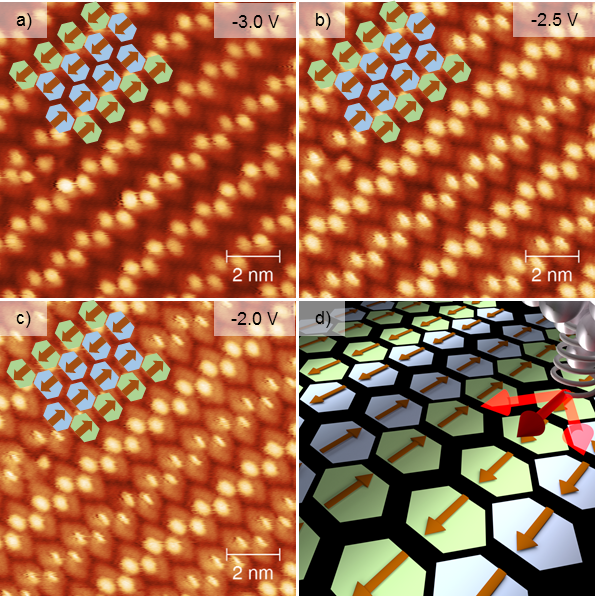
\includegraphics[width=0.7\textwidth]{./images/paper/helicene/fig4}
	\caption{Periodic change in contrast when $R_t = U_b / I$ changes. Cc-STM images (a-c) are acquired at a current set point of \SI{0.05}{\nano \ampere} but decreasing $U_b$ (given in upper right corner). Model representation (d) of possible dipole alignment between tip (red arrows) and molecular assembly (orange arrows). Dipole interaction strength changes with respect to their relative alignment which is responsible for the alternating contrast in cc-STM. The contrast difference quickly diminishes with increasing $U_b$ because electric dipole field scales with $~d^{-3}$.}
	\label{fig:hel-fig4}
\end{figure}

As the assembly is understood on the two silver substrates as well as on \textit{h}-BN, we take a closer look on the effects that are only visible on \textit{h}-BN. Varying the bias voltage ($U_b$) in constant current mode results in a periodic contrast pattern across the RT assembly of dcdb-[5]H on \textit{h}-BN (\autoref{fig:hel-fig4}). While at high $U_b$ the STM contrast resembles every strand with the same apparent height (a), lowering $U_b$ changes the apparent height of every second chain (b-c). Because these show the same dipole orientation of its constituents and therefor the same alternating pattern as the STM contrast, an interaction of a polar tip termination with the molecular dipole is likely. A tip termination with unfavorable tip-molecule interaction for one tip-dipole orientation will avoid regions with repulsive interaction. The accompanied increase in the tunneling distance results in chains being imaged in a darker contrast. The contrast is enhanced for the 180° rotated chains because here the interaction becomes attractive. An alternation of both effects results in the contrast pattern shown in \autoref{fig:hel-fig4}c. According to this, the modeled tip-dipole is assumed to be flexible (red arrow mounted on a spring in \autoref{fig:hel-fig4}d) and allowed to rotate in plane (semitransparent arrows) as it would result from the pickup of a molecule that is allowed to rotate around its helix axis. When $|U_b|$ is increased the increasing tip-sample distance quickly reduces the dipole-dipole interaction ($~d^{-3}$) and therefor a homogeneously distributed contrast across the chains as observed in \autoref{fig:hel-fig4}a. Please note that not only dipole-dipole interactions are present in the close proximity of functionalized tip and molecular assembly. With a molecule attached to the tip  interactions of the molecular helices are possible. The elevation of the distal parts in the helix of two neighboring chains is antiparallel and interaction with the tip may result in a similar contrast. Modification of the tip apex with [7]H is possible as reported in literature\cite{Ernst_Stereochemical_2016} and used for dimer-separation on a Cu(111) surface.

An electronic influence of the substrate on the occupied states of the molecule can be excluded as a reason for the contrast variation since the resulting pattern would show hexagonal symmetry as discussed in the following.

The inherent lattice mismatch between \textit{h}-BN and copper substrate results in an emerging moir\'e superstructure\cite{joshi_boron_2012}, dividing the surface in regions with smaller (wire) and larger surface potential (pore)\cite{Koitz_Structural_2013}. In \autoref{fig:hel-fig5}a-c pores are highlighted by dashed circles. Here molecular energy levels are shifted by the changing surface potential.\cite{Sushobhan_Control_2014} \autoref{fig:hel-fig5}a shows a STM topography where this electronic shift is visible as change in apparent height of the molecules. This can be explained by taking a closer look at energies close to the highest occupied molecular orbitals (HOMO) and lowest unoccupied molecular orbital (LUMO) states as shown in \autoref{fig:hel-fig5}b and c respectively. When tuning $U_b$ from \SIrange{0}{-3}{\volt} HOMO states appear first on the wire sites (\autoref{fig:hel-fig5}b) because on pore regions the HOMO is shifted further away from the fermi energy compared to the molecules on wire regions where occupied states are accessible first. When tuning $U_b$ from \SIrange{0}{3}{\volt} LUMO states are antithetically observed first on the pore sites (\autoref{fig:hel-fig5}c) where the larger surface potential shifts the unoccupied states closer to fermi.

\begin{figure} \centering
	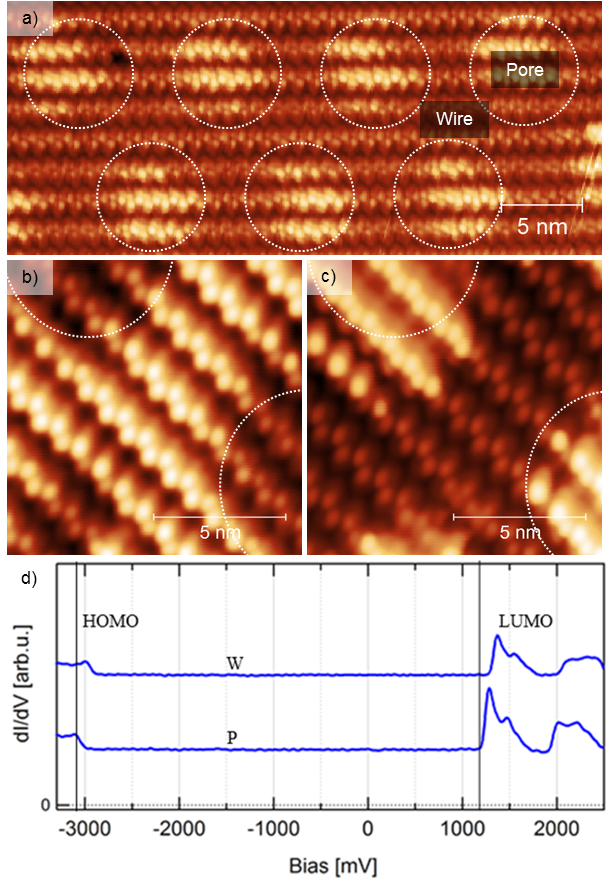
\includegraphics[width=0.7\textwidth]{./images/paper/helicene/fig5}
	\caption{STM topography with visible moir\'e protrusions (white dashed circles) recorded at \SI{1}{\volt}, \SI{0.05}{\nano \ampere} (a). STM topographies of HOMO (b, $U_b$=\SI{-3.1}{\volt}) and LUMO (c, $U_b$=\SI{1.2}{\volt}) states recorded at \SI{0.1}{\nano \ampere}. $U_b$ used for imaging is also indicated by black lines in the STS spectra (d) where HOMO/LUMO states and electronic gap are shown. Spectra labeled W(P) are recorded on a wire(pore) region of the moir\'e.}
	\label{fig:hel-fig5}
\end{figure}

Position depended differential STS (dI/dV) on molecules in the moir\'e unit cell shows this shift of HOMO and LUMO. On a pore site (P in \autoref{fig:hel-fig5}d) both states are shifted towards negative bias (to the left). This results in the HOMO (LUMO) being shifted further away (closer towards) the fermi level. The voltages at which STM was conducted in \autoref{fig:hel-fig5}b \& c are shown as black vertical lines limiting the electronic states contributing to the tunneling process to either include molecules on wire (\autoref{fig:hel-fig5}b) or pore (\autoref{fig:hel-fig5}c) regions. This is in agreement with the position depended emergence of the frontier orbitals in STM as discussed earlier. No hybridization with the metal substrate is observed, resulting in a large featureless electronic band gap of (\SI{4.4 \pm 0.1}{\eV}) and highlighting the effective electronic decoupling of the molecules by the \textit{h}-BN layer.


\section{Conclusions}

We contribute measurements on novel synthesized chiral molecules where chiral separation is overcome by intermolecular interactions. This is achieved by molecular design where a cyano group is added to the central ring of the helicene. On all substrates racemic assemblies are formed guided by the presence of the cyano group. Especially on Ag(111) dipole interactions of single strands favor the formation of paired strands along the high symmetry directions. Their assembly is stable upon annealing to 100°C and disintegrates quickly at higher temperatures. Here single molecules undergo a surface assisted cyclodehydrogenation using the silver surface as catalyst resulting in a new achiral compound. On Ag(100) more chain directions and setups can be reported, but only one where commensurate growth is observed. Furthermore it is shown that \textit{h}-BN is an adequate spacer layer to decouple dcdb-[5]H from the metallic support. Removing the metal substrate that facilitates growth along high symmetry directions results in extended island growth with no particular substrate registry. The isolating properties of \textit{h}-BN is indicated by unperturbed HOMO/LUMO states with a flat electronic gap measured in STS. \textit{h}-BN also templates the substrate’s surface potential directly transferring to HOMO/LUMO states, thus shifting them towards negative bias on pores and positive bias on wire regions. 
